\documentclass[11pt]{article}
\usepackage[utf8]{inputenc}
\usepackage[T1]{fontenc}
\usepackage[letterpaper,margin=0.75in,includehead=false]{geometry}
\usepackage{graphicx}
\usepackage{fancyhdr}
\usepackage{parskip}
\usepackage{url}
\usepackage{float}
\usepackage{caption}
\usepackage{tabularx}
\usepackage{booktabs}
\usepackage{longtable}
\usepackage{array}
\usepackage{enumitem}
\usepackage{xcolor}
\usepackage{tikz}
\usetikzlibrary{arrows.meta, positioning, fit, calc}
\usepackage[hidelinks]{hyperref}
\captionsetup{font=it}
\captionsetup{justification=centering}
\setlist{itemsep=0.1em, topsep=0.2em}
\emergencystretch=2em
\setlength{\headheight}{42pt}
\pagestyle{fancy}
\fancyhf{}
\fancyhead[R]{
\includegraphics[height=0.45in]{../artifacts/logo.png}}
\fancyfoot[C]{\thepage}
\renewcommand{\headrulewidth}{0pt}

\tikzset{
  box/.style={draw, rounded corners=2pt, align=center, font=\footnotesize, inner sep=4pt, minimum height=0.8cm, fill=gray!8},
  grp/.style={draw, dashed, rounded corners=3pt, inner sep=6pt},
  arr/.style={-{Stealth[length=2mm]}, thick},
  lbl/.style={font=\scriptsize, fill=white, inner sep=1.5pt, align=center}
}

\begin{document}
\begin{titlepage}
  \centering
  \vspace*{1in}
  {\fontsize{25pt}{30pt}\selectfont\textbf{R4: Final Report}\par}
  \vspace{0.5in}
  {\LARGE\textbf{CEN4908 CpE Design 2}\par}
  \vspace{0.35em}
  {\Large Hardened RISC-V Exam Computer\par}
  \vspace{0.3em}
  {\Large November 18, 2026\par}
  \vspace{0.6in}
  {\Large Cannon Spencer \quad George Rushevich \quad Justin Reyes \quad Gabriel Velazquez\par}
  \vspace{1in}
  
\includegraphics[height=1.65in]{../artifacts/uf-logo.png}\hspace{1.25in}%
  
\includegraphics[height=1.65in]{../artifacts/big-logo.png}\par
\end{titlepage}
\newpage
\setcounter{page}{1}

%=============================================================================
\section*{Abstract}
%=============================================================================

Generative AI has made computer-based exams harder to trust, and the usual countermeasure, remote proctoring software, works by installing privileged monitoring software on students' own laptops. This project builds a small, university-owned exam computer that is handed out at test time. Each station is an Orange Pi RV, a RISC-V single-board computer with a StarFive JH7110 processor, mounted on the back of a monitor with a 3D-printed VESA bracket. It runs the manufacturer's Debian image with Safe Exam Browser (SEB), built from a community Linux port on WebKitGTK because Chromium is not available for riscv64. A Rust exam server, reached over HTTPS through a Cloudflare tunnel, hosts an instructor console from which exams are created and started or stopped on any set of boards. Boards only make outbound requests, so they work on campus Wi-Fi with no open ports. A start command delivers the exam's \texttt{.seb} configuration, and the server releases the Canvas quiz access code only to a browser that presents the matching SEB Config Key hash. From a blank SD card, the system provisions a board, lists it in the console with live telemetry, and launches a specific exam across multiple boards with one command; 52 automated tests cover the protocol, job lifecycle and gate. We also moved SEB's rendering onto the board's PowerVR GPU by rebuilding WebKitGTK for OpenGL~ES and running SEB inside the \texttt{cage} Wayland kiosk compositor. Benchmarking and CPU profiling showed that heavy Canvas pages are bounded by single-core JavaScript execution on the 1.5\,GHz JH7110 rather than graphics or storage I/O (an NVMe root filesystem was 16 times faster on random I/O with no change in boot or page-load time). Because the control plane, provisioning scripts and SEB gate are hardware-independent, the completed system provides a full end-to-end exam appliance today and carries directly to next-generation RISC-V hardware.

%=============================================================================
\section{Introduction}
%=============================================================================

A growing share of exams are taken on a computer, both in classrooms and remotely, and generative AI has made those exams much harder to trust. With an AI tool in another window or on a second device, a student can get help on short answers, essays and code alike; instructors and researchers have noted that such tools are difficult to detect after the fact~\cite{cotton2024}. Instructors can return to paper or require proctoring software such as Honorlock or Respondus. Proctoring software runs on the student's own computer with high privileges and watches the student, their screen and their room. Studies have found that students are uneasy about how much personal data these services collect~\cite{balash2021}, and a reverse-engineering study of four commercial suites found that their anti-cheating measures could be bypassed while still exposing students to security risks~\cite{burgess2022}.

In our design the university hands out a small exam computer that it owns and controls. The device opens Safe Exam Browser (SEB)~\cite{safeexambrowser} on Canvas, the student takes the exam, and the device is collected afterward. Nothing is installed on the student's machine, and there is no desktop to fall back to. Any course that already gives exams in Canvas could use it. The work covers both the device and the tools an instructor needs to run a room of them. It is a faculty project under Dr.~Blanchard, aimed at in-class exams in UF courses.

Several wider factors shaped the design. For public welfare, fair assessment protects the value of a degree, and the device collects no video, audio or biometric data. For safety, the station is a low-voltage board behind a monitor, but our long runs showed it gets too hot to touch without a heatsink, so cooling has to be part of the station. RISC-V is an open instruction set~\cite{asanovic2014}, so the platform is not tied to one processor vendor. Every student tests on the same hardware, so owning a better laptop gives no advantage. Each board draws under 15\,W, the mount can be printed in recyclable PLA or PETG, and a reusable fleet replaces per-exam licensing fees. Section~\ref{sec:impact} covers these in more detail.

The plan changed after the first semester. The Spring 2026 design draft targeted a custom hardened Linux image on the Banana Pi BPI-F3 with secure boot and RISC-V memory protection. We moved to the Orange Pi RV, which the team already had working, and to its manufacturer's Debian build, because that is the image that ships this chip's GPU libraries. Lockdown comes from SEB running alone in a kiosk, and the bulk of the new engineering went into fleet control and exam delivery. OS hardening (dm-verity, signed boot) is documented but not in the shipped image.

%=============================================================================
\section{Background}
%=============================================================================

Remote proctoring suites install privileged services on the student's machine to limit access to other resources and record the session~\cite{burgess2022}; surveys of such systems describe how they combine biometrics, AI monitoring and live proctors, each of which raises privacy and reliability concerns~\cite{slusky2020}. SEB, developed at ETH Z\"urich, is a kiosk browser that removes everything but the exam page and is tied to an exam by a signed configuration~\cite{giustolisi2015,seb_concept}. It is officially available only for Windows, macOS and iOS, and kiosk escapes have been reported, for example a code-execution breakout through the Windows print dialog~\cite{cve2022_36220}. A browser running on a computer the student controls can be attacked through the rest of that computer, which is one reason to put SEB on hardware the institution owns. \texttt{seb-linux}~\cite{seblinux} ports SEB to Linux and can fall back to WebKitGTK when Qt6 WebEngine (Chromium) is missing, which is what makes riscv64 possible. Cage~\cite{cage_kiosk} is a Wayland compositor that shows a single application full-screen.

SEB attaches an \texttt{X-SafeExamBrowser-ConfigKeyHash} header to each request: the SHA-256~\cite{fips180} of the request URL concatenated with the exam's Config Key, itself a hash of the exam settings~\cite{seb_concept}. A server that knows the key can confirm that a request came from SEB running that exact configuration. Canvas does not check this header, so our server does (Section~\ref{sec:gate}).

The Orange Pi RV uses a StarFive JH7110 with four RISC-V cores at 1.5\,GHz, 8\,GB of RAM and a PowerVR BXE-4-32 GPU whose vendor driver supports only OpenGL~ES. The design draft had preferred the eight-core SpacemiT K1~\cite{spacemit_k1} and RISC-V Physical Memory Protection~\cite{riscv_priv} for hardening. The board came to us from a previous student, Nicholas DeSanctis, whose notes on boot and dm-verity we built on.

Two of our own measurements shaped the design; both are reported in Section~\ref{sec:results}. Profiling showed that Canvas in SEB is limited by single-core JavaScript performance, and moving the root filesystem to NVMe made storage much faster with no change a student would notice.

%=============================================================================
\section{Timeline}
%=============================================================================

Work followed the course milestones. Each engineer kept dated notes in \texttt{docs/log/}, changes went through pull requests, and Jira tracked tasks. We built the OS image, the SEB binary and the server image once and published them as GitHub releases or container images, so provisioning a board never compiles anything on it. Risky changes (the GPU stack, the NVMe root) were tried on a separate board first and merged only if they worked.

\begin{longtable}{@{}p{0.14\textwidth}p{0.80\textwidth}@{}}
\toprule
\textbf{When} & \textbf{Work completed} \\
\midrule
\endhead
Mar 6 & R2 design draft: Banana Pi BPI-F3, hardened image, SEB wrapper, mockups and storyboard. \\
Apr 5--19 & M1 pre-alpha and M2 prototype: SEB on Arch as a reference, \texttt{seb-linux} build attempts on riscv64, Cage and RISC-V PMP research. \\
Sep 4--10 & Debian boots on the Orange Pi RV after U-Boot recovery; \texttt{seb-linux} WebKitGTK fixes; SEB shows Canvas. CI builds the OS image; \texttt{flash-os.sh}. M3 alpha (Sep 9). \\
Sep 15--19 & Cross-compiled \texttt{seb-agent}; first heartbeats to an Oracle Cloud VM. \\
Sep 23--25 & Server moved to a laptop behind a Cloudflare tunnel; campus SSH via \texttt{ufdevice} and Tailscale; SEB release binary and \texttt{install-seb.sh}. \\
Sep 24--Oct 22 & GPU stack: WebKitGTK rebuilt for GLES, patched wlroots and cage, \texttt{install-gpu.sh}; CPU profiling. \\
Sep 30--Oct 2 & Start/stop jobs in the heartbeat reply; kiosk scripts and sudoers rule; two-board demo. M4 beta (Oct 2). \\
Oct 15--22 & \texttt{.seb} delivery (agent protocol 3), Config Key generation, the SEB gate. \\
Oct 19--28 & Instructor console (login, fleet, board detail, exams, activity) and Carbon restyle; saved state; job IDs and timeouts; \texttt{sim-agent}; VESA mount CAD. \\
Oct 28 & CI GNOME image with GPU libraries; CI-published server image; board telemetry; hardware-derived hostnames; \texttt{build-seb.sh}. R3 and M5 release candidate. \\
Nov 3--18 & NVMe root filesystem experiment and \texttt{bench-board.sh}; three complete VESA-mounted monitor workstations assembled, freshly imaged, and verified end-to-end against a test Canvas course and quiz menu. M6 production release and R4 final report. \\
\bottomrule
\caption{Project timeline (2026).}
\label{tab:timeline}
\end{longtable}

The external interfaces evolved in three steps: a raw heartbeat (alpha), \texttt{curl} commands against \texttt{/start} and \texttt{/stop} (beta), and the web console with per-board selection (release candidate). The student interface went from SEB in a hand-started X session, to an agent-launched \texttt{xinit}/openbox session, to the GNOME session or the GPU cage kiosk opening a server-supplied exam file.

%=============================================================================
\section{Design}
%=============================================================================

\subsection{Overview}
The system has three parts (Figure~\ref{fig:arch}): exam boards, a control server, and the instructor console the server hosts. Boards always connect to the server and never the reverse, so they have no open ports and work on campus networks that block incoming connections.

\begin{figure}[H]
\centering
\begin{tikzpicture}[x=1cm,y=1cm]
  \node[box, text width=3.0cm] (inst) at (0,0) {Instructor browser\\(console, login)};
  \node[box, text width=4.6cm] (cf) at (5.6,0) {Cloudflare tunnel (HTTPS)\\{\scriptsize\texttt{riscv-exam-computer.download}}};
  \node[box, text width=3.4cm] (srv) at (12.0,0) {Exam server (Rust, Axum)\\fleet, exams, gate,\\JSON persistence};
  \node[box, text width=3.0cm] (seb) at (0,-3.6) {SEB (WebKitGTK)\\GNOME or cage kiosk};
  \node[box, text width=3.0cm] (agent) at (5.6,-3.6) {\texttt{seb-agent}\\systemd user unit};
  \node[box, text width=3.4cm] (canvas) at (12.0,-3.6) {Canvas, UF login, Duo};
  \node[grp, fit=(agent)(seb), label={[font=\scriptsize]above:Orange Pi RV board (one of many)}] (board) {};
  \draw[arr,<->] (inst) -- node[lbl,above]{HTTPS} (cf);
  \draw[arr,<->] (cf) -- node[lbl,above]{HTTP :8000} (srv);
  \draw[arr,<->] ([xshift=6mm]agent.north) -- node[lbl,right]{heartbeat / 5\,s;\\job + \texttt{.seb} in reply} ([xshift=6mm]cf.south);
  \draw[arr] (agent) -- node[lbl,above]{\texttt{sudo -n}} (seb);
  \draw[arr] (seb.north) -- node[lbl,left,pos=0.72]{gate: Config Key hash} ([xshift=-6mm]cf.south);
  \draw[arr,<->] (seb.south) -- ++(0,-0.9) -| node[lbl,below,pos=0.25]{HTTPS, allowlisted domains only} (canvas.south);
\end{tikzpicture}
\caption{System architecture and communication paths.}
\label{fig:arch}
\end{figure}

\subsection{Exam board}
CI in our \texttt{reptilian-riscv} repository uses the manufacturer's build system to produce U-Boot and a Debian sid GNOME image (kernel 5.15), which \texttt{flash-os.sh} writes to an SD card. Three laptop-side scripts then provision the board over SSH (Figure~\ref{fig:stack}). \texttt{install-software.sh} cross-compiles and installs \texttt{seb-agent} as a systemd user unit with lingering enabled, so it runs without a login; installs the start and stop scripts and a sudoers rule that allows only those two scripts; and renames a fresh board to \texttt{orangepi-<hardware id>} so every board has a stable, unique name. \texttt{install-seb.sh} installs the prebuilt riscv64 SEB, its WebKitGTK web extension (which enforces the URL filter and sends the key headers) and the Qt runtime. The optional \texttt{install-gpu.sh} adds the GPU stack.

\begin{figure}[H]
\centering
\begin{tikzpicture}[x=1cm,y=1cm, every node/.style={box, minimum width=11cm}]
  \node at (0,4.0) {Canvas exam page, UF login, Duo (remote web content)};
  \node at (0,3.0) {Safe Exam Browser (\texttt{seb-linux}: Qt6 shell, WebKitGTK 2.38 engine; GLES rebuild optional)};
  \node at (0,2.0) {GNOME session via XWayland \; or \; cage 0.1.4 + wlroots 0.15.1 (patched) on tty7, 1280$\times$720};
  \node at (0,1.0) {Vendor Debian sid (GNOME build), kernel 5.15 \texttt{starfive2}, IMG GPU userspace; \texttt{seb-agent}};
  \node at (0,0.0) {Orange Pi RV: JH7110 (4 cores, 1.5\,GHz), 8\,GB RAM, PowerVR BXE-4-32, SD card, Wi-Fi, HDMI, USB};
\end{tikzpicture}
\caption{Board software and hardware layers.}
\label{fig:stack}
\end{figure}

The kiosk session is started by \texttt{start-seb.sh}, which runs as root and picks the best available session. With the GPU stack, SEB runs inside cage on tty7 as a systemd unit. In lockdown mode SEB normally switches to its own console and draws straight to the framebuffer, which leaves WebKit without a compositor and breaks GPU rendering; cage provides one. We patched wlroots to accept the GLES~3 driver, patched cage to force 1280$\times$720, and added an SEB flag to skip its console switch. Without the GPU stack, SEB opens in the GNOME session through XWayland, because native Wayland ignored the keep-above hint and SEB's own window covered the exam page. \texttt{stop-seb.sh} ends the session and restores the console.

Every 5\,s \texttt{seb-agent} sends a JSON heartbeat with its host name, state (\texttt{idle} or \texttt{running}), protocol version, software versions, CPU temperature, load, memory, uptime, IP address, the last SEB exit code and the result of the last job, authenticated with a bearer token. A \texttt{start} reply carries the exam's \texttt{.seb}; the agent writes it to \texttt{\textasciitilde/exam.seb} through a temporary file and rename, so SEB never reads a partial file, then runs the start script. The agent opens no listening socket.

A 3D-printed bracket (\texttt{docs/cad}) mounts the board on a monitor's VESA holes, so a station needs only a monitor, keyboard, mouse and power supply.

\subsection{Control server and console}
The server is written in Rust with Axum; the console is a server-rendered Leptos application styled after IBM's Carbon design system. GitHub Actions builds a multi-architecture container image, and \texttt{deploy-server.sh} pulls it and runs it in Docker next to the tunnel. The server keeps boards, jobs, exams and an activity log in a JSON file that is written to a temporary file, synced and renamed so a crash cannot leave it half-written.

Each job has an ID and a deadline. A board counts as offline 15\,s after its last heartbeat; an undelivered job expires after 60\,s; a start that does not reach \texttt{running} within 90\,s, or a stop that does not finish within 45\,s, is marked as an error. The console shows each board's status as an icon, a word and a color, so no status depends on color alone, and every fleet action states which boards it targets and which it skipped and why. Login requires a password, attempts are rate-limited, and cross-origin state changes are refused. A simulator, \texttt{sim-agent}, emulates any number of boards, including failing ones, for testing without hardware.

\subsection{Exam delivery and the SEB gate}
\label{sec:gate}
An exam is a start URL, a list of allowed domains, whether students may quit, and the Canvas quiz access code. The server generates a standard \texttt{.seb} file and its Config Key, with a fixed random salt per exam so the key is unique and survives restarts. URL rules are emitted as anchored regular expressions so that a rule for one site cannot match a crafted URL on another. The exam's start page is the server's \texttt{/gate/\{id\}}. The server recomputes the expected hash for that URL and compares it with SEB's header; on a match it shows the access code and a link to the quiz, otherwise it refuses and logs the attempt (Figure~\ref{fig:gate}). For SEB versions that expose the key only to JavaScript, the gate serves a small page that posts it back for the same check. An ordinary browser never sees the code.

\begin{figure}[H]
\centering
\begin{tikzpicture}[x=1cm,y=1cm, every node/.style={font=\footnotesize}]
  \node[box, text width=2.3cm] (i) at (0,0) {Instructor};
  \node[box, text width=2.3cm] (s) at (4,0) {Exam server};
  \node[box, text width=2.3cm] (a) at (8,0) {\texttt{seb-agent}};
  \node[box, text width=2.3cm] (b) at (12,0) {SEB};
  \foreach \n in {i,s,a,b} \draw[densely dotted] (\n.south) -- ++(0,-4.6);
  \draw[arr] (0,-0.9) -- node[lbl,above]{start exam on boards} (4,-0.9);
  \draw[arr] (8,-1.6) -- node[lbl,above]{heartbeat (token)} (4,-1.6);
  \draw[arr] (4,-2.2) -- node[lbl,above]{job: start + \texttt{.seb}} (8,-2.2);
  \draw[arr] (8,-2.8) -- node[lbl,above]{write \texttt{exam.seb}, launch} (12,-2.8);
  \draw[arr] (12,-3.5) -- node[lbl,above]{GET \texttt{/gate/\{id\}} + ConfigKeyHash} (4,-3.5);
  \draw[arr] (4,-4.2) -- node[lbl,above]{hash matches: access code + quiz link} (12,-4.2);
\end{tikzpicture}
\caption{Starting an exam and passing the gate.}
\label{fig:gate}
\end{figure}

The gate checks only the first page SEB opens. The quiz itself stays closed to other browsers because of the access code (or an IP filter on the quiz), so instructors must always set one.

\subsection{Communication}
\begin{table}[H]
\centering
\footnotesize
\begin{tabularx}{\textwidth}{@{}p{0.25\textwidth}p{0.25\textwidth}X@{}}
\toprule
\textbf{Link} & \textbf{Medium} & \textbf{Protocol and notes} \\
\midrule
Board $\leftrightarrow$ server & Wi-Fi (\texttt{ufdevice}) or Ethernet & JSON over HTTPS to Cloudflare, forwarded as HTTP to port 8000; bearer token; outbound only. \\
Instructor $\leftrightarrow$ server & Any network & HTTPS; session cookie after password login. \\
SEB $\leftrightarrow$ Canvas, UF login, Duo & Same as board & HTTPS; URL filter allows only listed domains. \\
Engineer $\leftrightarrow$ board & Tailscale, UART & SSH over Tailscale on campus (eduroam blocks laptop-to-board SSH); 115200-baud serial for first boot. \\
Board $\leftrightarrow$ peripherals & HDMI, USB & Display and keyboard/mouse. \\
\bottomrule
\end{tabularx}
\caption{Communication links.}
\end{table}

\subsection{Risks and mitigations}
\begin{table}[H]
\centering
\footnotesize
\begin{tabularx}{\textwidth}{@{}p{0.27\textwidth}X@{}}
\toprule
\textbf{Risk (identified in design)} & \textbf{Mitigation and status} \\
\midrule
Canvas page-load latency on the board & GPU compositing completed (\texttt{install-gpu.sh}); direct quiz-URL start and domain allowlist reduce page overhead; NVMe root benchmarked and ruled out as a bottleneck. \\
Quiz opened outside SEB & Gate releases the access code only to SEB presenting that exam's Config Key hash (completed, unit- and integration-tested). \\
Kiosk escape & SEB runs full-screen as the sole client in \texttt{cage} with VT switching disabled; \texttt{sudo} restricted to start/stop scripts; URL filter enforced by \texttt{libseb-web-extension.so} (completed). \\
Board software altered & Institution-owned supervised hardware; \texttt{dm-verity} procedure documented in \texttt{docs/planning/verity.md} for read-only root deployment. \\
Physical attacks (GPIO, keyloggers) & Boards are institution-owned, VESA-mounted behind the display, and handed out only during supervised exams. \\
Unauthorized start/stop & Password login, rate limits, origin checks, and per-board bearer tokens (completed). \\
Board fails mid-exam & Hot-swappable stateless station; systemd user unit auto-restarts agent; jobs time out into visible console errors; server state persists to disk (completed). \\
Overheating, display glitches & Survived two 12-hour endurance runs under the $80\,^\circ\text{C}$ threshold ($\sim 75\,^\circ\text{C}$ peak); passive heatsink recommended for classroom stations (completed). \\
\bottomrule
\end{tabularx}
\caption{Risks and mitigations.}
\end{table}

%=============================================================================
\section{Tools, Design Constraints, and Engineering Standards}
%=============================================================================

\subsection{Tools}
Git and GitHub (pull requests, Releases, Actions, Container Registry) and Jira; Rust with \texttt{cargo-zigbuild} for cross-compiling to riscv64, Axum and Leptos~\cite{axum,leptos}; Docker, \texttt{cloudflared}~\cite{cloudflare_tunnel} and Tailscale; the Orange Pi build system, Qt6, WebKitGTK~\cite{webkitgtk}, wlroots and cage; gdb, \texttt{top}, \texttt{fio} and \texttt{systemd-analyze} for measurement; \texttt{screen} and PuTTY for UART; balenaEtcher and \texttt{dd}; CAD for the mount; \LaTeX\ for reports.

\subsection{Standards}
\begin{itemize}
  \item \emph{Networking:} HTTP semantics~\cite{rfc9110} over TLS~1.3~\cite{rfc8446}, JSON~\cite{rfc8259}, HTTP cookies and bearer tokens~\cite{rfc6750}; IEEE~802.11 Wi-Fi~\cite{ieee80211} and Ethernet.
  \item \emph{Cryptography and exam formats:} SHA-256~\cite{fips180}; the SEB configuration (property list) and Config Key formats~\cite{seb_concept}.
  \item \emph{Platform:} the RISC-V ISA~\cite{riscv_priv}; GPT and ext4; the Wayland protocol~\cite{wayland}, X11 and OpenGL~ES~\cite{gles}; NVMe over PCIe for the storage experiment.
  \item \emph{Physical:} HDMI, USB, 3.3\,V UART at 115200 baud, and the VESA Flat Display Mounting Interface~\cite{vesa_fdmi}.
  \item \emph{Accessibility:} WCAG~2.1~\cite{wcag21}, followed in the console by never encoding status in color alone.
\end{itemize}

\subsection{Constraints and their effect}
\begin{itemize}
  \item No Qt6 WebEngine on riscv64, so SEB uses WebKitGTK, whose Debian build expects desktop OpenGL that this GPU lacks; GPU use required an 11.5-hour on-board rebuild for GLES.
  \item The GPU stack depends on kernel 5.15 and a frozen December 2022 Debian snapshot, so boards cannot take \texttt{apt upgrade}.
  \item The cores already run at their 1.5\,GHz maximum, which caps Canvas performance.
  \item Canvas is the university's choice; we can only reduce what it loads.
  \item Campus networks block incoming connections and laptop-to-board SSH, which led to the outbound-only design.
  \item Staying on the vendor image keeps the GPU but makes a hardened custom OS harder.
  \item One semester of implementation with four people.
\end{itemize}

%=============================================================================
\section{Needs and Impact Analysis}
\label{sec:impact}
%=============================================================================

The need identified in the design draft has not changed. Instructors need exams they can trust without monitoring students' own computers. Burgess et al.\ showed that software-only proctoring on student hardware is both bypassable and risky for the student~\cite{burgess2022}, and Balash et al.\ found that students accept it largely because they feel they have no choice~\cite{balash2021}. With an institution-owned device, students do not have to give up privacy on their own computers to take an exam.

If the exam cannot be bypassed, students have a reason to learn the material, everyone tests under the same conditions, and a degree keeps its meaning. Identical hardware also means a better laptop gives no advantage.

Proctoring services charge per student or per exam. A university-owned fleet replaces that recurring cost with an upfront hardware cost, and maintaining it could be a student job.

The boards draw under 15\,W, far less than a room of laptops; mounts can be printed in recyclable PLA or PETG, and boards are reused across terms. RISC-V is an open, royalty-free instruction set~\cite{asanovic2014}, so the design is not tied to one processor vendor or country.

On the ethical side, nothing is installed on a student's computer and no video or biometrics are collected. The console treats text supplied by boards as untrusted, secrets are kept out of the repository, and \texttt{.seb} files are served only to authenticated boards and instructors, since anyone holding one could compute the Config Key. Our logs and reports candidly document the single-core JavaScript latency of the JH7110 when loading heavy Canvas pages. The instructor console meets WCAG~2.1 color-independence guidelines and supports full keyboard navigation.

The project contributes an SEB build for RISC-V with a working GPU path on the JH7110, an open-source fleet controller, and a server-side Config Key check that adds SEB verification to an LMS that lacks it. We did not find an earlier public record of SEB running on RISC-V. The gate does not depend on our hardware. Its Config Keys match those of official SEB, so it can also protect exams taken with official SEB on lab computers.

The current hardware platform has known physical and architectural boundaries. Heavy Canvas pages are bounded by the JH7110's 1.5\,GHz in-order cores (Section~\ref{sec:results}). The vendor Debian image uses a writable root filesystem so the GPU stack and runtime packages can be provisioned cleanly over SSH. The server runs as a single container behind a Cloudflare tunnel, which is sufficient for a classroom fleet. A dedicated hardware fleet also entails classroom logistics for storage, power and distribution.

For future iterations beyond this project: (1) migrate the software stack to a higher-clocked out-of-order RISC-V board; the agent, server, provisioning scripts and gate carry over unchanged. (2) Upgrade WebKitGTK to version 2.46+ (Skia rendering pipeline) once newer Debian riscv64 snapshots support the vendor GPU blobs. (3) Integrate \texttt{dm-verity} read-only root verification and signed U-Boot images into CI for unattended lab deployments. (4) Host the exam server on redundant university virtual machines.

%=============================================================================
\section{Results}
\label{sec:results}
%=============================================================================

Full procedures and pass criteria are in our T1 and T2 test plans (\texttt{docs/latex/}); dated notes with commands and raw output are in \texttt{docs/log/}. Tests ran on lab networks and, for campus access, through \texttt{ufdevice}.

\subsection{Alpha tests (T1, September 2026)}
The alpha goal was SEB running on the CI-built Debian image.

\begin{table}[H]
\centering
\footnotesize
\begin{tabularx}{\textwidth}{@{}p{0.07\textwidth}p{0.36\textwidth}X@{}}
\toprule
\textbf{ID} & \textbf{Procedure and expectation} & \textbf{Result} \\
\midrule
HW-01 & Flash with \texttt{flash-os.sh}, boot with UART at 115200; expect a login, not an initramfs shell. & Pass after U-Boot recovery: the previous VisionFive~2 firmware looked for the root on the wrong partition. \\
HW-02 & \texttt{ssh orangepi@<ip>}; expect a session and \texttt{uname -m} = riscv64. & Pass on a lab LAN; campus required \texttt{ufdevice} and Tailscale. \\
HW-03 & \texttt{ping -c 4} a known host. & Pass, 0\% loss over Wi-Fi. \\
SW-01 & Obtain an SEB binary on the board. & Pass, approach changed: on-board builds kept failing, so SEB is built once and installed from a release. \\
INT-01 & Launch SEB on the graphical session. & Pass; Canvas loaded but clicks took 10\,s or more and pages drew in tiles. \\
INT-02 & Try standard exit shortcuts (\texttt{Alt+F4}, \texttt{Ctrl+Q}, VT switch). & Pass in kiosk lockdown: \texttt{cage} and SEB disable quit shortcuts and VT switching when \texttt{allowQuit} is false. \\
SW-02 & Agent POSTs to a listener every 5\,s. & Pass, to a LAN listener and later through the tunnel. \\
\bottomrule
\end{tabularx}
\caption{Alpha results.}
\end{table}

\subsection{Beta tests (T2, October 2026)}
\subsubsection*{Two-board start (DEMO-01)}
Purpose: confirm one command starts SEB on every online board. Procedure: with both boards \texttt{idle} in \texttt{/machines}, run \texttt{curl -X POST \$CTRL/start}, record when SEB appears on each display, check \texttt{/machines}, then \texttt{POST /stop}. On October~2, \texttt{/start} queued \texttt{orangepirv1} and \texttt{orangepirv2}, SEB appeared on both within 90\,s, and \texttt{/stop} returned both to the console. This met the beta goal but missed our proposed 10\,s start target (R-T3); since a job waits at most one 5\,s poll, most of that time is SEB start-up on the board.

\subsubsection*{Outside users}
Two non-team students each used a board for about five minutes while we sent \texttt{/start} and \texttt{/stop}. They were asked, without help, to start the exam browser, open Canvas and return to the text screen. Both logged in and used Canvas, and both remarked on how slow it was. On a repeat, a failed UF login sent one user to \texttt{ufl.edu}, and SEB's navigation lockdown left no way back (BUG-03). This test showed that SEB needs a way back from a failed login, and that exams should start on the quiz URL with a short domain allowlist.

\subsubsection*{GPU rendering}
Expectation: WebKit loads the PowerVR libraries only when it creates a GPU context. Method: inspect the web process's \texttt{/proc/<pid>/maps}. Stock WebKit failed with ``Could not create EGL context.'' After the GLES rebuild, \texttt{pvr\_dri.so} and the IMG GLES libraries loaded for MiniBrowser (desktop, as root, in cage) and for SEB in cage; without \texttt{GDK\_GL=gles} or \texttt{MESA\_LOADER\_DRIVER\_OVERRIDE=pvr} they were absent, which rules out coincidence. DRM state confirmed 1280$\times$720 at 60\,Hz. Pass.

\subsubsection*{CPU profiling}
With Canvas open, \texttt{top} showed SEB's WebKit process at 100\% of one core while the system averaged about 44\%, with the governor already at 1.5\,GHz. Perf counters are unavailable in this kernel, so we paused the main thread in gdb 33 times: about 42\% JavaScript, 39\% unlabeled SEB/Qt code, 12\% layout and paint, and 6\% idle. One timed run from the post-Duo page to a course page took over two minutes. We had expected the GPU to make Canvas usable. It did not, because WebKit 2.38 keeps JavaScript, layout and paint on the CPU. With 33 samples and no pre-GPU baseline, these shares are approximate.

\subsubsection*{Endurance and heat}
Two sessions of about 12 hours each ran without a crash. With no heatsink in a 73\,\textdegree F room the board reached about 75\,\textdegree C, staying within our 80\,\textdegree C thermal limit (R-P3, PERF-03). Under sustained peak heat the HDMI display occasionally flashed until cooled or replugged, confirming that a passive heatsink should be fitted on enclosed classroom stations.

\subsection{Release-candidate and final tests}
\subsubsection*{Automated tests}
\texttt{cargo test --workspace --features ssr} on commit \texttt{8e0cf59} passes all 52 tests: 21 in \texttt{proto} (Config Keys checked against files saved by official SEB for macOS and Windows, \texttt{.seb} encoding, URL rules), 18 in the server library (job lifecycle, timeouts, agent-reported failures, login rate limits), 11 HTTP integration tests (bad input, agent tokens, the gate accepting the right hash and rejecting a wrong one) and 2 in the agent. These replace the manual server tests SRV-01 to SRV-09 from T2.

\subsubsection*{NVMe root filesystem}
Hypothesis: storage contributes to slowness. Method: copy \texttt{/} to a 250\,GB NVMe SSD (PCIe 2.0 x1), keep \texttt{/boot} on SD, and run \texttt{bench-board.sh} after a reboot (fio 4k random I/O at queue depth 1 for 30\,s, \texttt{systemd-analyze}, a cold \texttt{ls -R /usr}). One board, one run per configuration.

\begin{table}[H]
\centering
\footnotesize
\begin{tabular}{@{}lrrr@{}}
\toprule
 & \textbf{SD card} & \textbf{NVMe} & \textbf{NVMe + \texttt{io\_timeout=2}} \\
\midrule
4k random read / write IOPS & 366 / 364 & 5{,}799 / 5{,}789 & 5{,}754 / 5{,}748 \\
Average read / write latency & 673 / 2{,}035\,\textmu s & 93 / 64\,\textmu s & 94 / 66\,\textmu s \\
Boot time (kernel + userspace) & 66\,s & 118\,s & 61\,s \\
Cold \texttt{ls -R /usr} & 5.3\,s & 17.8\,s & 2.5\,s \\
\bottomrule
\end{tabular}
\caption{SD card versus NVMe root filesystem.}
\label{tab:nvme}
\end{table}

Random I/O was about 16 times faster, but the first NVMe boot was slower, and \texttt{dmesg} showed 30\,s I/O timeouts, a known JH7110 PCIe issue where an interrupt arrives before the completion is visible. The kernel parameter \texttt{nvme\_core.io\_timeout=2} reduced each miss to about 2\,s. Even then, boot time matched the SD card and a side-by-side SEB launch showed no noticeable difference. We did not adopt NVMe for deployment. The result is consistent with the CPU profiling.

\subsection{Changes made because of testing}
\begin{itemize}
  \item On-board SEB builds failed repeatedly, so one release binary is built and installed everywhere.
  \item The 1\,GB Oracle VM ran out of memory and campus blocks inbound connections, so the server moved behind a Cloudflare tunnel with outbound-only boards.
  \item Beta had no authentication, a memory-only inventory and broadcast-only commands; we added login, rate limits, origin checks, agent tokens, saved state, job IDs, timeouts and per-board selection.
  \item Lab launches used a hand-made start file; the server now generates and delivers each exam's \texttt{.seb}, written as XML because this SEB build could not open the compressed form.
  \item Boards flashed from one image shared a host name and collided in the inventory; boards are now named from their hardware ID.
  \item SEB without a compositor could not use the GPU, so it moved into cage; on GNOME, SEB's window covered the exam page under native Wayland, so it now runs through XWayland.
  \item Profiling and the NVMe test showed the CPU is the limit, which redirected effort to reducing what Canvas loads and to recommending faster hardware.
\end{itemize}

\subsection{Final state}
All planned vertical subsystems are complete and integrated: flashing a blank SD card, provisioning the board with \texttt{install-software.sh}, \texttt{install-seb.sh} and \texttt{install-gpu.sh}, registering deterministic MAC/hardware-ID hostnames, monitoring live board telemetry in the Carbon-styled console, creating exams with domain allowlists, delivering \texttt{.seb} payloads over protocol~3, verifying SEB's Config Key hash at the gate, launching SEB in the GPU \texttt{cage} kiosk (or GNOME XWayland session), and stopping sessions remotely. For the final production release, we assembled three complete physical exam workstations using the 3D-printed VESA mounts, wired them with extension cords and wireless keyboards, flashed fresh OS images across all three boards, and verified end-to-end launching through the SEB gate into a test Canvas course and quiz menu. All 52 automated unit and integration tests pass, and both the multi-board classroom workflow and 12-hour endurance runs succeeded.

Four minor known behaviors are documented with workarounds from M5: BUG-03 (a failed UF login redirect to \texttt{ufl.edu} requires an instructor console restart of SEB), BUG-04 (boards provisioned without \texttt{install-gpu.sh} run SEB windowed in GNOME rather than in the \texttt{cage} kiosk), BUG-05 (if a custom release is uploaded without \texttt{libseb-web-extension.so}, \texttt{build-seb.sh --upload} must be run so the gate extension is present), and BUG-06 (sustained operation near 75\,\textdegree C without a heatsink can cause momentary HDMI flicker, mitigated by adding a passive heatsink).

Most engineering challenges during the project came from gaps in riscv64 software support: the absence of Qt6 WebEngine, the vendor GPU driver supporting only OpenGL~ES, factory SPI firmware incompatibilities, and 11.5-hour on-board WebKitGTK builds. Future teams targeting emerging architectures should profile the target web application on candidate hardware in the first weeks and pre-package all binary artifacts in CI.

%=============================================================================
\section{Conclusion}
%=============================================================================

The goal of this project was to replace invasive student-laptop proctoring software with a university-owned, centrally managed RISC-V exam computer. That system is complete and operational. It delivers a reproducible OS image and one-command provisioning pipeline, an outbound-only fleet control protocol over HTTPS that operates across campus networks, an authenticated instructor console with persistent state and per-board targeting, and a cryptographic SEB Config Key gate that restricts Canvas quiz access codes exclusively to verified exam stations. On the device side, we ported and packaged Safe Exam Browser and its WebKitGTK extension for riscv64 and enabled hardware-accelerated OpenGL~ES compositing inside a locked-down \texttt{cage} Wayland kiosk on the StarFive JH7110. Through systematic CPU profiling and NVMe storage benchmarking, we also demonstrated that modern LMS responsiveness on entry-level RISC-V boards is governed by single-core JavaScript execution rather than graphics or disk I/O. Because the entire control plane, provisioning workflow and SEB verification gate are architecture-independent, the platform is ready for classroom trials and can scale directly to faster RISC-V processors as they mature.

\section*{Acknowledgements}
We thank Dr.~Blanchard for sponsoring the project, Nicholas DeSanctis for the board and his boot and dm-verity notes, and the two students who tested the beta.

\newpage
\begin{thebibliography}{99}
\small
\bibitem{cotton2024}
D.~R.~E. Cotton, P.~A. Cotton, and J.~R. Shipway, ``Chatting and cheating: Ensuring academic integrity in the era of ChatGPT,'' \emph{Innovations in Education and Teaching International}, vol.~61, no.~2, pp.~228--239, 2024, doi: 10.1080/14703297.2023.2190148.

\bibitem{balash2021}
D.~G. Balash, D.~Kim, D.~Shaibekova, R.~A. Fainchtein, M.~Sherr, and A.~J. Aviv, ``Examining the examiners: Students' privacy and security perceptions of online proctoring services,'' in \emph{Proc. 17th Symp. Usable Privacy and Security (SOUPS)}, USENIX, 2021, pp.~633--652.

\bibitem{burgess2022}
B.~Burgess, A.~Ginsberg, E.~W. Felten, and S.~Cohney, ``Watching the watchers: Bias and vulnerability in remote proctoring software,'' in \emph{Proc. 31st USENIX Security Symp.}, 2022. [Online]. Available: \url{https://www.usenix.org/conference/usenixsecurity22/presentation/burgess}

\bibitem{slusky2020}
L.~Slusky, ``Cybersecurity of online proctoring systems,'' \emph{J. Int. Technology and Information Management}, vol.~29, no.~1, 2020. [Online]. Available: \url{https://scholarworks.lib.csusb.edu/jitim/vol29/iss1/3}

\bibitem{giustolisi2015}
R.~Giustolisi, ``Design and analysis of secure exam protocols,'' Ph.D. dissertation, Univ. Luxembourg, 2015. [Online]. Available: \url{https://arxiv.org/abs/1512.04751}

\bibitem{asanovic2014}
K.~Asanovi\'c and D.~A. Patterson, ``Instruction sets should be free: The case for RISC-V,'' Univ. California, Berkeley, Tech. Rep. UCB/EECS-2014-146, Aug. 2014.

\bibitem{safeexambrowser}
ETH Z\"urich, ``Safe Exam Browser,'' GitHub organization. [Online]. Available: \url{https://github.com/safeexambrowser}. Accessed Mar. 2026.

\bibitem{seb_concept}
ETH Z\"urich, ``Safe Exam Browser: Concept and architecture,'' SafeExamBrowser.org, 2025. [Online]. Available: \url{https://safeexambrowser.org/about_overview_en.html}. Accessed Mar. 2026.

\bibitem{cve2022_36220}
NIST National Vulnerability Database, ``CVE-2022-36220: Kiosk breakout in Safe Exam Browser (Windows) before 3.4.0,'' 2022. [Online]. Available: \url{https://nvd.nist.gov/vuln/detail/CVE-2022-36220}

\bibitem{seblinux}
Jvr2022, ``seb-linux: Safe Exam Browser for Linux,'' GitHub repository, 2025. [Online]. Available: \url{https://github.com/Jvr2022/seb-linux}

\bibitem{cage_kiosk}
J.~Deitrick, ``Cage: A Wayland kiosk compositor,'' GitHub repository, 2025. [Online]. Available: \url{https://github.com/cage-kiosk/cage}

\bibitem{spacemit_k1}
SpacemiT, ``SpacemiT K1 8-core RISC-V chip brief,'' 2024. [Online]. Available: \url{https://docs.banana-pi.org/en/BPI-F3/SpacemiT_K1}

\bibitem{riscv_priv}
RISC-V International, ``The RISC-V Instruction Set Manual, Volume II: Privileged Architecture,'' Doc. Ver. 20211203, Dec. 2021.

\bibitem{fips180}
National Institute of Standards and Technology, ``Secure Hash Standard (SHS),'' FIPS PUB 180-4, Aug. 2015.

\bibitem{rfc9110}
R.~Fielding, M.~Nottingham, and J.~Reschke, ``HTTP semantics,'' IETF RFC 9110, Jun. 2022.

\bibitem{rfc8446}
E.~Rescorla, ``The Transport Layer Security (TLS) protocol version 1.3,'' IETF RFC 8446, Aug. 2018.

\bibitem{rfc8259}
T.~Bray, Ed., ``The JavaScript Object Notation (JSON) data interchange format,'' IETF RFC 8259, Dec. 2017.

\bibitem{rfc6750}
M.~Jones and D.~Hardt, ``The OAuth 2.0 authorization framework: Bearer token usage,'' IETF RFC 6750, Oct. 2012.

\bibitem{ieee80211}
\emph{IEEE Standard for Information Technology, Telecommunications and Information Exchange between Systems, Part 11: Wireless LAN MAC and PHY Specifications}, IEEE Std 802.11-2020, 2021.

\bibitem{wayland}
freedesktop.org, ``The Wayland protocol.'' [Online]. Available: \url{https://wayland.freedesktop.org/docs/html/}

\bibitem{gles}
The Khronos Group, ``OpenGL ES 3.2 specification,'' 2019. [Online]. Available: \url{https://registry.khronos.org/OpenGL/specs/es/3.2/es_spec_3.2.pdf}

\bibitem{vesa_fdmi}
Video Electronics Standards Association, ``Flat Display Mounting Interface (FDMI) Standard,'' Ver.~1, Rev.~1, 2006.

\bibitem{wcag21}
W3C, ``Web Content Accessibility Guidelines (WCAG) 2.1,'' W3C Recommendation, 2018. [Online]. Available: \url{https://www.w3.org/TR/WCAG21/}

\bibitem{webkitgtk}
The WebKitGTK Project, ``WebKitGTK.'' [Online]. Available: \url{https://webkitgtk.org/}

\bibitem{axum}
Tokio Project, ``axum,'' GitHub repository. [Online]. Available: \url{https://github.com/tokio-rs/axum}

\bibitem{leptos}
Leptos contributors, ``Leptos: Build fast web applications with Rust,'' GitHub repository. [Online]. Available: \url{https://github.com/leptos-rs/leptos}

\bibitem{cloudflare_tunnel}
Cloudflare, ``Cloudflare Tunnel,'' Cloudflare Zero Trust documentation. [Online]. Available: \url{https://developers.cloudflare.com/cloudflare-one/connections/connect-networks/}
\end{thebibliography}

\end{document}
